%% FullCourse_10Lecs -- Lecture 6, Topic 6.5b: KFE side of MFG + Lab Preview
%% Source: ./archive_pre_split/Lec06_HA_Models.tex (section 10 second half + section 11)
%% Sub-split: original T5 (sections 10-11) exceeded 30-page ceiling at 31 pages.
%% Split into T5a (MFG motivation + HJB) and T5b (KFE + deep MFG + lab preview).
%% FullCourse-only content: Mean-Field Games section (not present in MiniCourse).

%% Shared preamble for the FullCourse_10Lecs topic decks.
%%
%% Each topic .tex \input's this file, then defines its own \title, \date
%% override (if any), \graphicspath, and \begin{document}.
%%
%% Reconstructed verbatim from the inlined copy preserved in
%% Lec10_Case_Studies/Lec10_T8_Case6_DeepRamsey.tex (lines 23-190), which is
%% explicitly annotated there as "from ../shared_preamble.tex, copied verbatim".
%% Base preamble matches MiniCourse_8hr/Slides/shared_preamble.tex; this version
%% additionally provides \sectiondivider, the conceptbox/cautionbox/examplebox/
%% takeawaybox tcolorboxes, and \compacttables used across the split decks.

\documentclass[10pt,english,aspectratio=169]{beamer}

\usepackage{ae,aecompl}
\usepackage[T1]{fontenc}
\usepackage{textcomp}
\usepackage[utf8]{inputenc}
\usepackage{babel}
\usepackage{datetime2}

\setcounter{secnumdepth}{3}
\setcounter{tocdepth}{3}

\usepackage{amsmath, amssymb, amsthm, graphicx}
\usepackage{booktabs, multirow}
\usepackage{tikz}
\usepackage{pgfplots}
\pgfplotsset{compat=1.16}
\usepackage[most]{tcolorbox}
\tcbuselibrary{skins, breakable, theorems}
\usepackage{listings}
\usepackage{xcolor}

\lstset{
  basicstyle=\ttfamily\small,
  keywordstyle=\color{blue!80!black}\bfseries,
  commentstyle=\color{green!50!black}\itshape,
  stringstyle=\color{orange!80!black},
  backgroundcolor=\color{gray!8},
  frame=single,
  rulecolor=\color{gray!40},
  breaklines=true,
  showstringspaces=false,
  numbers=none,
}

\lstdefinestyle{pythonstyle}{
    language=Python,
    basicstyle=\ttfamily\footnotesize,
    keywordstyle=\color{blue!80!black}\bfseries,
    commentstyle=\color{green!50!black}\itshape,
    stringstyle=\color{orange!80!black},
    frame=single,
    breaklines=true,
    showstringspaces=false,
    numbers=left,
    numbersep=5pt,
    numberstyle=\tiny\color{gray},
    backgroundcolor=\color{gray!8},
    rulecolor=\color{gray!40}
}

\ifx\hypersetup\undefined
  \AtBeginDocument{%
    \hypersetup{bookmarks=false,breaklinks=true,pdfborder={0 0 0},colorlinks=true,
      linkcolor=DarkText,urlcolor=RedTitle}%
  }
\else
  \hypersetup{bookmarks=false,breaklinks=true,pdfborder={0 0 0},colorlinks=true,
    linkcolor=DarkText,urlcolor=RedTitle}%
\fi

\makeatletter
\newcommand\makebeamertitle{%
  \begin{frame}[plain]
    \vspace*{1.0cm}
    \centering
    {\usebeamerfont{title}\usebeamercolor[fg]{title}\inserttitle\par}
    \vspace{1.0cm}
    {\usebeamerfont{author}\usebeamercolor[fg]{author}\insertauthor\par}
    \vspace{0.2cm}
    {\usebeamerfont{date}\usebeamercolor[fg]{date}\insertdate\par}
  \end{frame}}%
\AtBeginDocument{%
  \let\origtableofcontents=\tableofcontents
  \def\tableofcontents{\@ifnextchar[{\origtableofcontents}{\gobbletableofcontents}}
  \def\gobbletableofcontents#1{\origtableofcontents}%
}

\usetheme{metropolis}
\usefonttheme{professionalfonts}

\definecolor{LightGray}{RGB}{230,230,230}
\definecolor{RedTitle}{RGB}{0,0,200}
\definecolor{VeryLightGray}{RGB}{245,245,245}
\definecolor{DarkText}{RGB}{0,0,0}

\setbeamercolor{background canvas}{bg=white}
\setbeamercolor{title}{fg=RedTitle}
\setbeamercolor{author}{fg=DarkText}
\setbeamercolor{date}{fg=DarkText}
\setbeamercolor{frametitle}{bg=VeryLightGray,fg=DarkText}
\setbeamercolor{normal text}{fg=DarkText}
\setbeamerfont{title}{size=\large}

\setbeamersize{text margin left=5mm, text margin right=5mm}
\addtobeamertemplate{frametitle}{}{\vspace{-0.5em}}
\newcommand{\reducevspace}{\vspace{-0.5cm}}

% Shared section divider and box styles for split topic decks.
\newcommand{\sectiondivider}[2]{%
\begin{frame}[plain,noframenumbering]
\begin{center}
\vfill
{\Large\textbf{#1}\par}
\vspace{0.35cm}
{\normalsize #2\par}
\vfill
\end{center}
\end{frame}
}

\newtcolorbox{conceptbox}[1][]{
  colback=blue!3,
  colframe=RedTitle!55,
  boxrule=0.35mm,
  arc=1mm,
  left=2mm,
  right=2mm,
  top=1mm,
  bottom=1mm,
  #1
}
\newtcolorbox{cautionbox}[1][]{
  colback=red!3,
  colframe=red!50!black,
  boxrule=0.35mm,
  arc=1mm,
  left=2mm,
  right=2mm,
  top=1mm,
  bottom=1mm,
  #1
}
\newtcolorbox{examplebox}[1][]{
  colback=green!3,
  colframe=green!45!black,
  boxrule=0.35mm,
  arc=1mm,
  left=2mm,
  right=2mm,
  top=1mm,
  bottom=1mm,
  #1
}
\newtcolorbox{takeawaybox}[1][]{
  colback=VeryLightGray,
  colframe=RedTitle!55,
  boxrule=0.35mm,
  arc=1mm,
  left=2mm,
  right=2mm,
  top=1mm,
  bottom=1mm,
  #1
}
\newcommand{\compacttables}{\renewcommand{\arraystretch}{1.15}}

\setbeamertemplate{navigation symbols}{}
\setbeamertemplate{footline}{%
  \hfill%
  \usebeamercolor[fg]{page number in head/foot}%
  \usebeamerfont{page number in head/foot}%
  \insertframenumber\,/\,\inserttotalframenumber\kern1em\vskip2pt%
}

\makeatother

\author{Zhigang Feng}
% "date with time": compile timestamp so each build is identifiable.
\date{\today\ \DTMcurrenttime}


\graphicspath{{./pic/}{../../MiniCourse_8hr/Slides/Module2_DL_RL_Macro/pic/}{../}}

\title[AI for Econ Research]{AI for Economic Research: Dynamic Models, Language, and Agents\\
Lecture 6.5b: KFE, Deep MFG, and Lab Preview}

\begin{document}

\makebeamertitle

%=============================================================================
\begin{frame}{Topic 6.5b Agenda}
\begin{enumerate}
  \item \textbf{Mean-Field Games (continued)} --- KFE, discretisation, master equation, deep MFG
  \medskip
  \item \textbf{Lab Preview and Wrap-up}
\end{enumerate}
\medskip
\textit{Arc: T1 Aiyagari + computation $\to$ T2a Why ML / Euler $\to$ T2b Global DNN $\to$ T3 KS / DeepHAM $\to$ T4 DEQN / OLG $\to$ T5a MFG HJB $\to$ \textbf{T5b MFG KFE + Lab}}
\end{frame}

%=============================================================================
\section{Mean-Field Games (continued)}
% FullCourse-only

\begin{frame}{The Kolmogorov forward (Fokker--Planck) equation}
For the time-dependent density $g_i(a,t)$:
\[
\partial_t g_i(a,t) \;=\; -\partial_a\!\big(s_i(a,t)\, g_i(a,t)\big)
- \lambda_i\, g_i(a,t) + \lambda_{-i}\, g_{-i}(a,t).
\]
\medskip

\begin{itemize}
\item First term: \emph{drift} --- mass moves at speed $s_i(a,t)$ along the $a$-axis.
\item Second term: \emph{Poisson outflow} from state $i$ at rate $\lambda_i$.
\item Third term: \emph{Poisson inflow} from the other state at rate $\lambda_{-i}$.
\medskip
\item Boundary: at the borrowing limit $a = \underline a$, mass cannot leak below; we impose a reflecting boundary.
\medskip
\item Well-posed under standard conditions (Achdou et al. 2022).
\end{itemize}
\end{frame}

\begin{frame}{Reading the KFE: economic intuition}
\begin{itemize}
\item \textbf{Drift term}: the cross-section flows to the right when households are saving ($s_i > 0$) and to the left when they are dissaving.
\medskip
\item \textbf{Jump terms}: at every point in $a$, mass leaks from state $i$ at rate $\lambda_i$ and arrives from $-i$ at rate $\lambda_{-i}$. The two states ``trade'' agents.
\medskip
\item \textbf{Boundary at $\underline a$}: reflecting boundary --- mass that hits the borrowing constraint cannot continue leftward; instead it accumulates at $\underline a$ for as long as $s_i(\underline a) \leq 0$.
\medskip
\item \textbf{Total mass conserved}: $\int g_1 + \int g_2 = 1$ at all times.
\medskip
\item Analogy: water flowing through two interconnected tanks with leaks at known rates.
\end{itemize}
\end{frame}

\begin{frame}{Stationary KFE}
At the stationary equilibrium ($\partial_t = 0$):
\[
0 \;=\; -\partial_a\!\big(s_i(a)\, g_i(a)\big) - \lambda_i\, g_i(a) + \lambda_{-i}\, g_{-i}(a),
\quad i = 1, 2.
\]
\medskip

\begin{itemize}
\item Two coupled ODEs in $g_1, g_2$, plus the normalisation $\int g_1 + \int g_2 = 1$.
\medskip
\item Reflecting boundary at $\underline a$, integrability at $a \to \infty$.
\medskip
\item Standard discretisation gives a sparse linear system $A^\top g = 0$ where $A$ is the discretised HJB infinitesimal generator (next slide).
\end{itemize}
\end{frame}

\begin{frame}{Discretisation and the upwind scheme}
\begin{center}
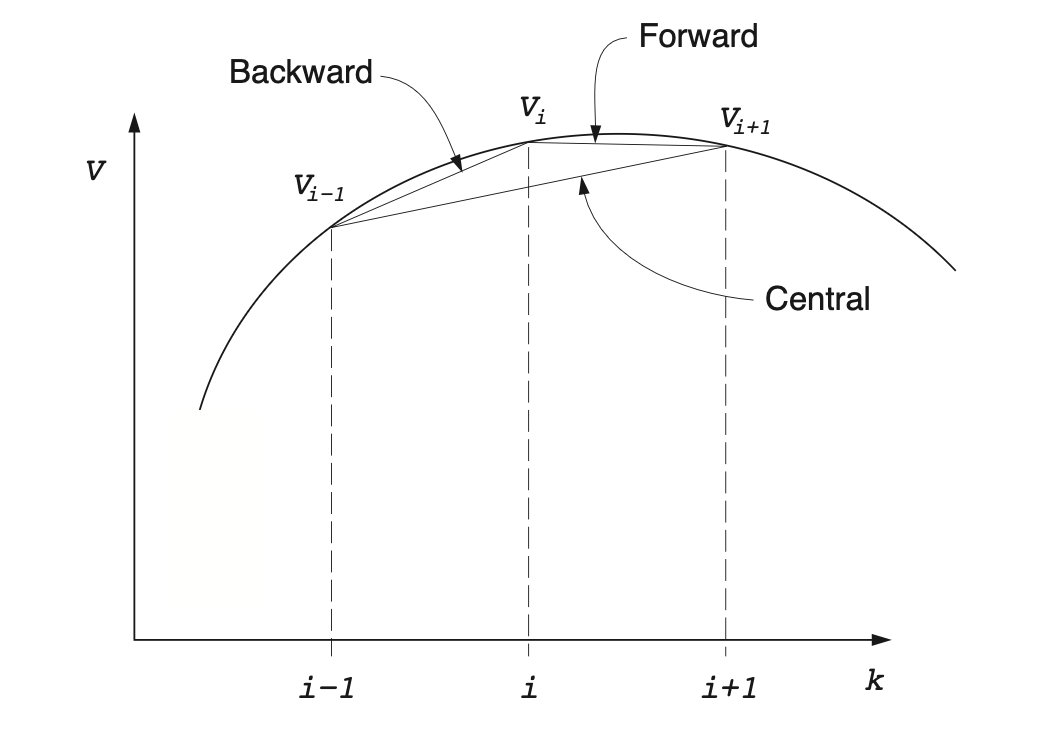
\includegraphics[width=0.6\textwidth]{vp}
\end{center}
\vspace{-0.3em}
\begin{itemize}
\item Discretise $a$ on a grid $\{a_1, \ldots, a_N\}$. The HJB needs an approximation of $v_i'(a)$.
\item \textbf{Upwind scheme}: pick the forward or backward difference depending on the \emph{sign of the optimal drift}:
\[
v_i'(a_j) \approx \begin{cases}
(v_i(a_{j+1}) - v_i(a_j))/\Delta a & \text{if } s_i(a_j) > 0 \\
(v_i(a_j) - v_i(a_{j-1}))/\Delta a & \text{if } s_i(a_j) < 0
\end{cases}
\]
\item Provably stable (Barles--Souganidis 1991); without upwinding, the scheme is unstable.
\end{itemize}
\end{frame}

\begin{frame}{HJB and KFE: $A$ vs.\ $A^\top$ duality}
After upwind discretisation, the HJB takes the form
\[
\rho\, \mathbf v \;=\; \mathbf u(\mathbf c) + A(\mathbf v)\, \mathbf v,
\]
where $A(\mathbf v) \in \mathbb{R}^{2N\times 2N}$ is the discretised infinitesimal generator (sparse, tridiagonal-plus-jumps).
\medskip

The discretised stationary KFE is
\[
\mathbf 0 \;=\; A(\mathbf v)^{\top}\, \mathbf g.
\]
\medskip
\begin{itemize}
\item The \emph{same} matrix $A$ generates both equations: HJB on the right, KFE on the left (transpose).
\medskip
\item This duality is at the heart of the Achdou et al.\ approach: solving HJB gives you the KFE almost for free.
\end{itemize}
\end{frame}

\begin{frame}{Putting it all together: outer fixed point on $r$}
\begin{enumerate}
\item Guess $r$.
\medskip
\item Solve HJB by iterating
\[
\rho \mathbf v - A(\mathbf v)\mathbf v \;=\; \mathbf u(\mathbf c)
\]
to find $\mathbf v^*, \mathbf c^*, A^*$.
\medskip
\item Solve KFE: find $\mathbf g^*$ in the null space of $A^{*\top}$, normalised to $\mathbf 1^\top \mathbf g^* = 1$.
\medskip
\item Aggregate: $K^* = \sum_j a_j \big(g^*_{1,j} + g^*_{2,j}\big)$.
\medskip
\item Update $r$ from the firm FOC at $K^*$ and iterate until convergence.
\end{enumerate}
\medskip

This is the Achdou--Lasry--Lions--Moll algorithm for continuous-time HA models. It is fast, accurate, and (with deep learning) extends to high-dimensional state spaces.
\end{frame}

\begin{frame}{Transition dynamics: forward--backward system \textsc{(advanced --- skip on first pass)}}
For non-stationary problems (e.g.\ MIT shocks, business cycles), HJB and KFE become time-dependent and the system is \emph{forward--backward}:
\[
\begin{cases}
-\partial_t v_i + \rho v_i \;=\; \max_c\,\{\cdots\}, & \text{(backward in time)}\\[0.4em]
\partial_t g_i \;=\; -\partial_a(s_i g_i) - \lambda_i g_i + \lambda_{-i} g_{-i}. & \text{(forward in time)}
\end{cases}
\]
\medskip
\begin{itemize}
\item Boundary in time: $v_i(\cdot, T) = $ terminal condition (often the stationary $v_i^*$); $g_i(\cdot, 0) = $ initial condition.
\medskip
\item Numerical scheme: \emph{shooting} or \emph{Newton's method} on the residuals --- iterate backward HJB given $g$, then forward KFE given $v$, until self-consistent.
\end{itemize}
\end{frame}

\begin{frame}{Master equation: distribution as state \textsc{(advanced --- skip on first pass)}}
\begin{itemize}
\item The master equation is a single equation that encodes both HJB and KFE simultaneously, with the \emph{distribution itself} as a state variable.
\medskip
\item Schematically:
\[
\rho\, U(x, m) \;=\; H\!\big(x, \nabla_x U(x,m), m\big) + \int \nabla_m U(x,m)(y)\, \mathcal L^* m(y)\, dy,
\]
where $U$ is the value function defined on the product space (individual state, distribution) and $\mathcal L^*$ is the dual generator on the distribution.
\medskip
\item This is an infinite-dimensional PDE on the Wasserstein space of probability measures.
\medskip
\item Practical use: linearisation around the stationary equilibrium gives a tractable system for solving HA models with aggregate shocks (Bilal 2023; Alvarez--Lippi 2022).
\end{itemize}
\end{frame}

\begin{frame}{Deep learning for MFG}
\begin{itemize}
\item Classical numerical schemes (upwind, finite differences) suffer in high-dimensional state spaces.
\medskip
\item \textbf{Deep neural networks for MFG}:
  \begin{itemize}
  \item Parameterise $v(x, m)$ and $m(x)$ by NNs.
  \item Train by minimising the residual of the HJB and the KFE jointly.
  \item Use Monte Carlo sampling instead of grids.
  \end{itemize}
\medskip
\item Recent progress (Carmona--Lauri\`ere 2021, Lauri\`ere et al.\ 2022) shows that deep MFG solvers can handle 10--20 dimensional state spaces that are completely out of reach for grid methods.
\medskip
\item These methods unify the discrete-time RL approaches (DeepHAM, DEQN) with the continuous-time PDE perspective.
\end{itemize}
\end{frame}

\begin{frame}{MFG $\leftrightarrow$ HA models: the link}
\begin{itemize}
\item Discrete-time Aiyagari is the natural \emph{discretisation} of continuous-time MFG with idiosyncratic Poisson income.
\medskip
\item Krusell--Smith with aggregate uncertainty corresponds to MFGs with a \emph{common noise} (the aggregate shock).
\medskip
\item In both formulations:
  \begin{itemize}
  \item Optimal individual behaviour depends on the cross-sectional distribution.
  \item The cross-sectional distribution evolves under optimal behaviour.
  \item Equilibrium is a fixed point of this circular dependence.
  \end{itemize}
\medskip
\item MFG provides the cleanest mathematical formalism, while RL/DL provide the computational engine.
\medskip
\item The two approaches are now converging: deep MFG solvers borrow heavily from RL; modern deep RL borrows from continuous-time control theory.
\end{itemize}
\end{frame}

%=============================================================================
\section{Lab Preview and Wrap-up}

\begin{frame}{Lab06 preview: Krusell--Smith via Deep Equilibrium Nets}
\begin{itemize}
\item In the 1-hour lab you will train a Deep Equilibrium Net to solve the Krusell--Smith (1998) economy in PyTorch.
\medskip
\item Notebook: \texttt{Lab06\_KS\_HA.ipynb} (in this folder).
\medskip
\item By the end of the lab you will:
  \begin{itemize}
  \item Initialise the model from a steady state computed via the sequence-Jacobian (SSJ) toolbox.
  \item Build a PyTorch policy network for the savings rate.
  \item Run the cloud-of-economies training loop.
  \item Visualise the trained policy and the loss curves.
  \item Diagnose convergence and accuracy.
  \end{itemize}
\medskip
\item Hardware: a single GPU (Colab T4 / V100) is comfortable; CPU also works for short runs.
\medskip
\item \textit{Forward pointer:} the cloud-simulation pattern in this lab ($N$ parallel economies, batched Euler-residual minimisation) reappears in Lec07 as cloud-of-prompts batch processing in LLM pretraining --- same hardware-utilisation argument, different objective.
\end{itemize}
\end{frame}

\begin{frame}{Lab06 step-by-step}
\textbf{Part 1.} Initialise via sequence-Jacobian:
\begin{itemize}
\item Solve the steady state to get asset and employment grids, transition matrices, $K_{ss}, \mu_{ss}$.
\end{itemize}
\medskip

\textbf{Part 2.} PyTorch implementation:
\begin{itemize}
\item Define the policy network (3 hidden layers, Mish, sigmoid output).
\item Encode the budget constraint inside the network.
\item Wrap the model physics (transition dynamics) as a class.
\end{itemize}
\medskip

\textbf{Part 3.} The training loop (cloud simulation):
\begin{itemize}
\item Simulate $N$ parallel economies.
\item Compute the Euler-residual loss.
\item Backprop and Adam update.
\item Transport the distribution forward (no grad).
\end{itemize}
\medskip

\textbf{Part 4.} Analysis:
\begin{itemize}
\item Plot the loss history (log scale).
\item Plot policy functions; check Euler errors.
\end{itemize}
\end{frame}

\begin{frame}{Lab06: expected-output checkpoint}
After Part 3 (training) and before Part 4 (analysis), check the lab is healthy:
\medskip
\begin{itemize}
\item \textbf{Training loss curve.} Monotone decreasing on log scale; Euler residual $\lesssim 10^{-4}$ on a held-out validation sample.
\medskip
\item \textbf{Learned savings policy.} $\sigma_\theta(a, e; Z, K)$ monotone in $a$; employed agents save more than unemployed at the same $a$ (precautionary motive).
\medskip
\item \textbf{Aggregate consistency.} $K_n$ across cloud copies stays within $\pm 5\%$ of the SSJ steady-state $K_{ss}$; fan plot narrows toward steady state, not diverging.
\end{itemize}
\medskip
If any of these look wrong, the trainer has not converged --- inspect learning rate, batch size, and cloud size $N$ before reading the policy plots.
\end{frame}

\begin{frame}{Optional follow-up: Lab12\_OLG.ipynb}
\begin{itemize}
\item Once you finish the KS lab, you may want to explore \texttt{Notebooks/Lab12\_OLG.ipynb}.
\medskip
\item This notebook implements OLG with aggregate uncertainty using JAX and stabilising homotopies (Brumm--Kubler--Scheidegger 2023).
\medskip
\item Highlights:
  \begin{itemize}
  \item Two-stage homotopy: first solve a capital-only model, then introduce bonds.
  \item JAX \texttt{jit} compilation for fast training-simulation episodes.
  \item Detailed pedagogical commentary inside the notebook.
  \end{itemize}
\medskip
\item Useful preparation for research projects involving life-cycle, fiscal policy, or asset-pricing applications.
\end{itemize}
\end{frame}

\begin{frame}{Suggested readings}
\begin{description}
\item[\textit{Aiyagari family.}] Bewley (1986); Huggett (1993, \emph{JEDC}); Aiyagari (1994, \emph{QJE}); Stokey, Lucas \& Prescott (1989, Harvard UP); Carroll (2006, \emph{Econ.\ Letters}).
\medskip
\item[\textit{Aggregate uncertainty.}] Krusell \& Smith (1998, \emph{JPE}); Kaplan, Moll \& Violante (2018, \emph{AER}).
\medskip
\item[\textit{Deep-learning HA.}] Han, Yang \& E (2021 preprint, arXiv:2112.14377; \emph{Quantitative Economics} 17:297--341, 2026); Azinovic, Gaegauf \& Scheidegger (2022, \emph{IER}); Brumm, Kubler \& Scheidegger (2023, working paper).
\medskip
\item[\textit{Continuous-time + MFG.}] Achdou, Han, Lasry, Lions \& Moll (2022, \emph{REStud}); Lasry \& Lions (2007, \emph{Japanese J.\ Math.}); Huang, Malham\'e \& Caines (2006, \emph{Communications in Information and Systems} 6(3):221--252).
\end{description}
\end{frame}

\begin{frame}{Bridge: from HA models to LLMs (Lec07)}
\begin{itemize}
\item \textit{Same building blocks:} neural function approximation (T2a \texttt{ValueNet}, T3 DeepHAM, T4 DEQN) reappears as transformer blocks parameterising $\log p(\text{token} \mid \text{context})$.
\medskip
\item \textit{Same training discipline:} sampling-based losses (Euler residuals, fictitious play) become next-token cross-entropy on cloud-of-prompts batches.
\medskip
\item \textit{Same actor--critic structure:} Lec05 T3 policy gradient comes back as RLHF (Lec07 T3) --- policy $=$ LLM, reward $=$ preference model trained on human comparisons.
\medskip
\item \textit{Same scaling story:} cloud-simulation of $N$ economies in the Lab06 DEQN trainer is the same parallelism that batches $N$ documents in LLM pretraining.
\end{itemize}
\medskip
Lec07 changes the \emph{object} (text rather than wealth distributions) but reuses every algorithmic primitive from Lec05 and Lec06.
\end{frame}

\begin{frame}{Recap of Lecture 6}
\begin{itemize}
\item \textbf{Aiyagari--Bewley--Huggett}: incomplete-markets HA model and stationary equilibrium; existence/uniqueness via Feller, mixing, monotonicity.
\medskip
\item \textbf{Classical computation}: nested fixed-point on $r$; VFI on the household, eigenvector for the distribution, bisection on the price.
\medskip
\item \textbf{Why ML?} Curse of dimensionality once we add aggregate shocks, multiple assets, or life-cycle structure.
\medskip
\item \textbf{Deep dynamic programming}: policy/value networks, Euler residual losses, actor--critic.
\medskip
\item \textbf{DeepHAM and DEQN}: two leading deep-learning solutions for KS.
\medskip
\item \textbf{OLG with aggregate uncertainty}: homotopy-stabilised JAX training.
\medskip
\item \textbf{Mean-Field Games}: continuous-time formulation, HJB+KFE, deep MFG solvers as the unifying frontier.
\medskip
\item \textbf{Next lecture}: Large Language Models --- a different but equally fast-moving deep-learning frontier.
\end{itemize}
\end{frame}

\end{document}
